
\documentclass[journal, onecolumn]{IEEEtran}[10pt]

% correct bad hyphenation here
\hyphenation{op-tical net-works semi-conduc-tor}

\usepackage{graphicx}
\usepackage{subfig}
\usepackage{amssymb}
\usepackage{amsmath} 

\begin{document}

% Do not put math or special symbols in the title.
\title{Final Project of ELEC5470 FALL 2017 \\ Optimization in Image Deblurring \\ Initial Proposal}

\author{Xiaoyun~Yuan,~20322404}


% The paper headers
\markboth{ELEC5470 Final Project Xiaoyun Yuan}%
% The only time the second header will appear is for the odd numbered pages
{}
% make the title area
\maketitle

% As a general rule, do not put math, special symbols or citations
% in the abstract or keywords.
\begin{abstract}
In this report , we present some representative image deblurring algorithms and the convex/non-convex optimization techniques used in these papers. 
\end{abstract}

% Note that keywords are not normally used for peerreview papers.
\begin{IEEEkeywords}
Optimization, Image Deblurring, Prior 
\end{IEEEkeywords}

% For peerreview papers, this IEEEtran command inserts a page break and
% creates the second title. It will be ignored for other modes.
\IEEEpeerreviewmaketitle

\section{Introduction}
Nowadays, smart phone has become the digital hub of everyone's daily life, and camera is one of the most important modules on smart phones. However, limited by the space of smart phones, the smart phone camera optic system is often very simple and CMOS size is usually very small. That means the image quality is easily affected environment, for example, low light condition leads to severe noise, camera shaking and long exposure time causes uncomfortable blur effect. In this report, we focus on how to remove the image blur effects caused by camera shaking.

Image deblurring is a fundamental computer vision research problem. Now, there are two different ways to solve the image deblurring problem: 1) traditional convolutional model approach; 2) neural network approach. In this report, we mainly focused on the first approach and give some brief introductions of the second approach.

In traditional convolutional model, the image blur effect is expressed by $2D$ convolution:
\begin{equation}
\mathbf{b} = \mathbf{l} \otimes \mathbf{k} + \mathbf{n},
\label{eqn:convolutional_blur_model}
\end{equation}
where $\mathbf{b}$, $\mathbf{l}$ and $\mathbf{k}$ are the blurry image, latent sharp/unblurred image and blur kernel respectively. $\mathbf{n}$ denotes the noise. The blur kernel $\mathbf{k}$ is usually expressed by a small matrix which is related to the camera shaking trajectory, as shown in the Fig.~\ref{fig:convolutional_blur_model}. Because the 2D convolution is difficult to handle, Eqn.~\ref{eqn:convolutional_blur_model} is often written in frequency domain:
\begin{equation}
\mathcal{F}(\mathbf{b}) = \mathcal{F}(\mathbf{l}) \cdot \mathcal{F}(\mathbf{k}) + \mathcal{F}(\mathbf{n}),
\label{eqn:convolutional_blur_model_frequency}
\end{equation}
where $\mathcal{F}(\cdot)$ denotes the Fourier transform.
\begin{figure}[h!]
\centering
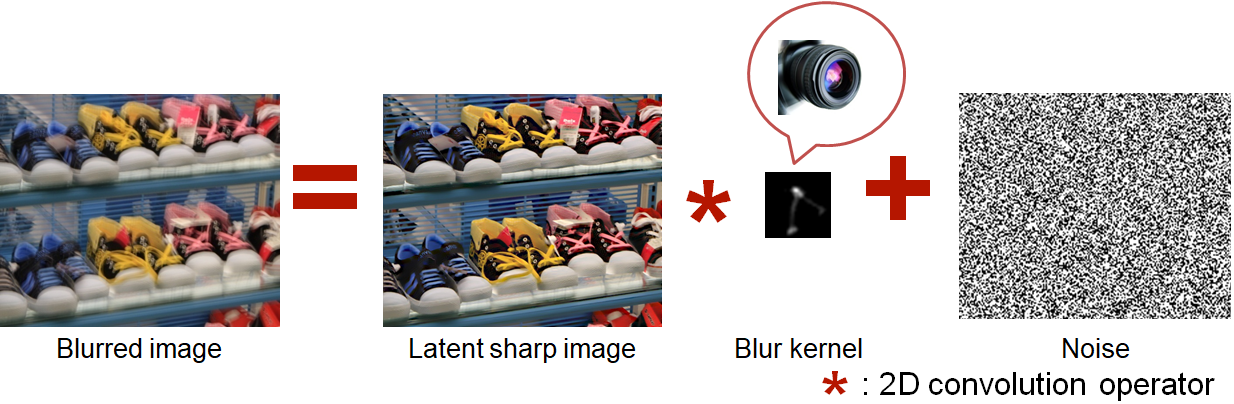
\includegraphics[width = 1\textwidth]{pic/convolutional_model.png}
\caption{Image Convolutional Blur Model}
\label{fig:convolutional_blur_model}
\end{figure}

The deblurring problem can be divide into two kinds: 1) non-blind deblurring: only $\mathbf{l}$ is unknown, use existing $\mathbf{k}$ to solve latent sharp image $\mathbf{l}$; 2) blind deblurring: both $\mathbf{l}$ and $\mathbf{k}$ are unknown. 

\section{Conclusion}
The conclusion goes here.



% by themselves when using endfloat and the captionsoff option.
\ifCLASSOPTIONcaptionsoff
  \newpage
\fi


% http://www.michaelshell.org/tex/ieeetran/bibtex/
\bibliographystyle{IEEEtran}
% argument is your BibTeX string definitions and bibliography database(s)
\bibliography{reference}


% that's all folks
\end{document}


